% Chapter Template

\chapter{Ensayos y resultados} % Main chapter title

\label{Chapter4} % Change X to a consecutive number; for referencing this chapter elsewhere, use \ref{ChapterX}
En el Salar del Llullaillaco se delimitó el área de estudio mediante un polígono SIG y se generaron mosaicos mensuales por misión Landsat (mediana de reflectancia) para homogenizar la observación y comparar interanualmente. El análisis se enfocó en la laguna central —la de mayor recurrencia hídrica y relevancia ecológica— y se cartografió el agua con NDWI utilizando un umbral de 0.2, validado para ambientes altoandinos. Se emplearon Landsat 5 TM (principal antes de 2011) y Landsat 8 OLI (2013–2024), limitando Landsat 7 ETM+ por la falla SLC (post mayo de 2003), lo que dejó una brecha 2012–2013. Para construir series mensuales continuas se aplicó una estrategia híbrida: interpolación en vacíos cortos y promedio estacional histórico en vacíos largos. Las pruebas de raíz unitaria mostraron estacionariedad en ONI, SOI y MEI, y una tendencia en el Área que requirió diferenciación; con ello, los modelos SARIMA lograron buen desempeño, destacándose \textit{Área\_diff} por su robustez. Finalmente, los análisis VAR y la causalidad de Granger evidenciaron interdependencia entre los índices ENSO y un papel especialmente influyente del SOI sobre la superficie de agua, reforzando la relación entre variabilidad atmosférica regional y dinámica hidrológica del salar.


%----------------------------------------------------------------------------------------
%	SECTION 1
%----------------------------------------------------------------------------------------

\section{Construcción de la serie temporal continua}

El primer paso consistió en evaluar la disponibilidad de imágenes por año y por variable 
derivada, lo que permitió identificar períodos con escasa cobertura. En particular, se 
consideraron como años incompletos aquellos con más de un 50\% de vacíos de información, 
es decir, con menos de seis meses de observaciones válidas en alguna de las series 
analizadas. Este diagnóstico reveló brechas significativas en ciertos intervalos, como 
el año 2012, donde no se registraron imágenes útiles.

A partir de este análisis se plantearon dos estrategias para construir una serie mensual 
continua de superficie de agua:

\begin{enumerate}
    \item Escenario estricto (descartar años incompletos): en este enfoque se 
    eliminaron directamente los años con cobertura insuficiente, priorizando la calidad 
    de los datos a costa de acortar la longitud de la serie temporal. 

    \item Estrategia híbrida de imputación: se diseñó un procedimiento de dos 
    etapas que permite conservar toda la serie completa entre 1984 y 2022: 
    \begin{itemize}
        \item Para \textit{brechas cortas} (menores o iguales a cinco meses) se aplicó 
        interpolación temporal, de modo de mantener la coherencia local de las 
        observaciones.
        \item Para \textit{brechas largas} (como años completos sin datos), se recurrió a 
        la imputación estacional, reemplazando los valores ausentes por el promedio 
        histórico de cada mes. De esta forma se preserva la estacionalidad propia de la 
        serie, evitando la introducción de sesgos por valores promedio anuales.
    \end{itemize}
\end{enumerate}


La estrategia híbrida permitió mantener la continuidad de la serie completa, a la vez 
que redujo el impacto de los vacíos extensos. Por su parte, el escenario estricto se 
conservó como ejercicio de sensibilidad metodológica, contrastando la robustez de los 
resultados frente a diferentes tratamientos de los faltantes. En la figura ~\ref{fig:ts_final} se muestran las series temporales resultantes.


\begin{figure}[ht]
        \centering
        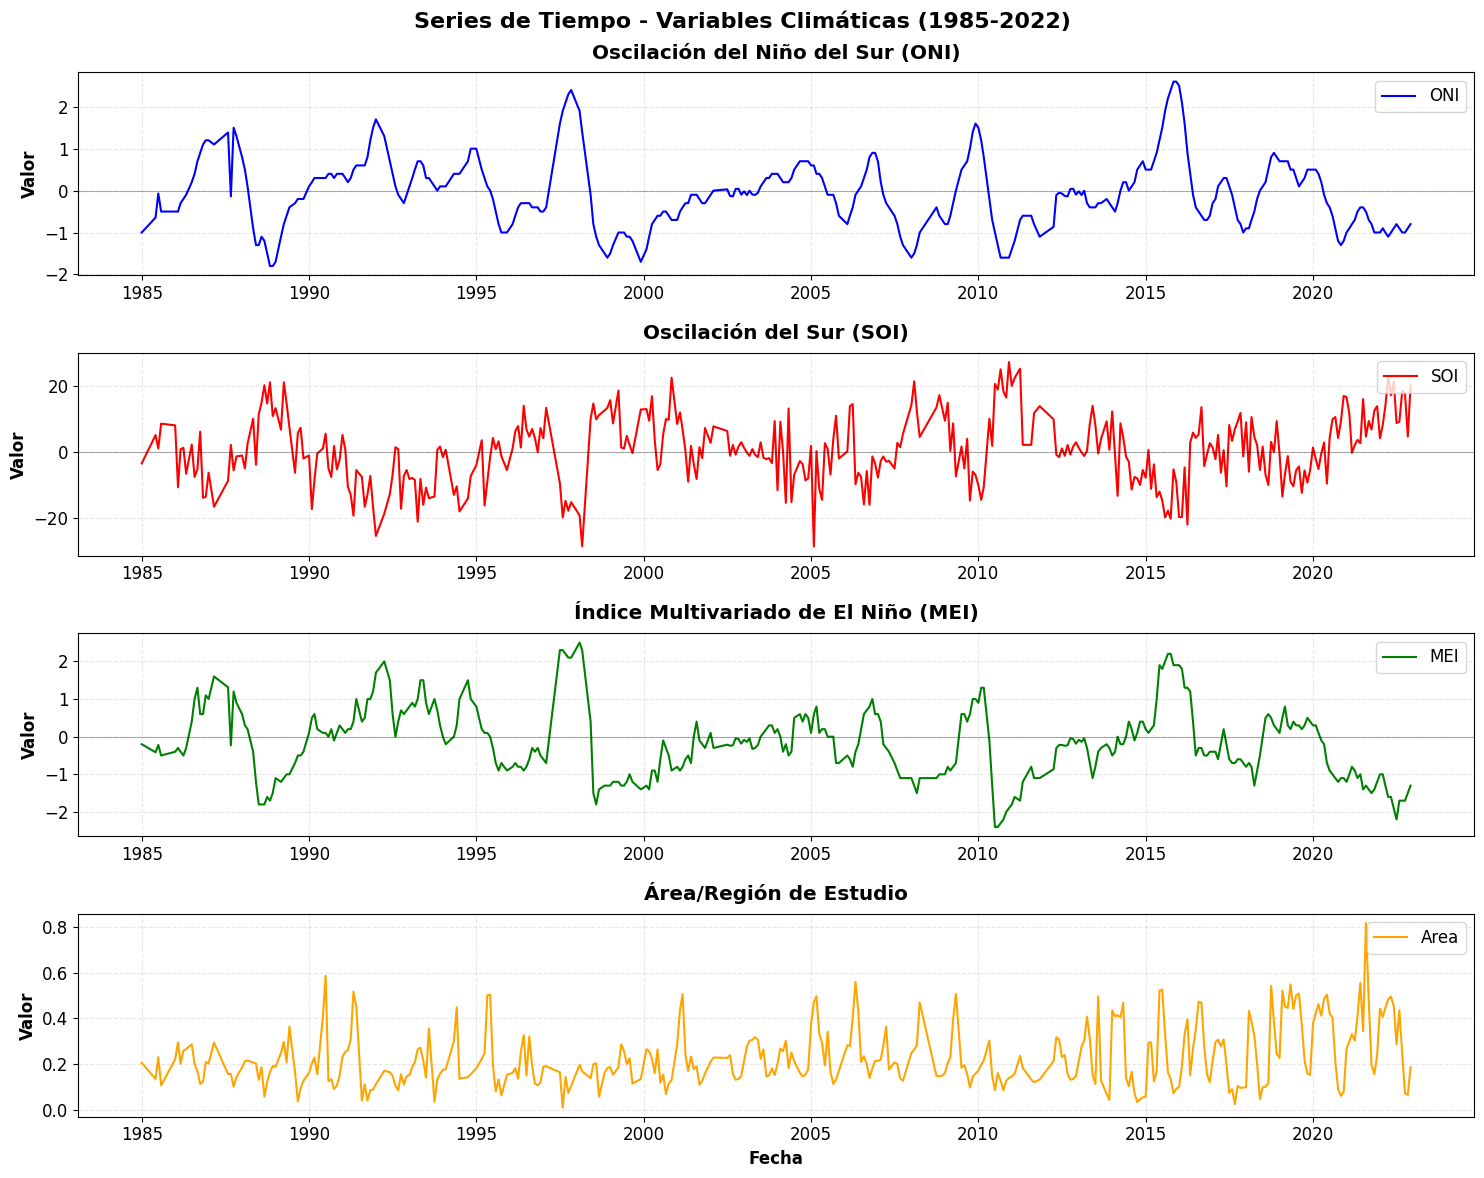
\includegraphics[scale=.32]
        {Figures/ts_final.png}
        \caption{Series Temporales Procesadas.}
        \label{fig:ts_final}
\end{figure}

\newpage
\section{Exploración y tratamiento de las Series Temporales}

\subsection{Raíces Unitarias}

Antes de la aplicación de modelos autorregresivos, se realizó un análisis visual de las 
series para explorar posibles tendencias o comportamientos no estacionarios. De manera 
preliminar, se observaron los siguientes patrones:

\begin{itemize}
    \item Serie Área (superficie de agua): muestra una tendencia descendente a lo 
    largo del período analizado, disminuyendo de valores cercanos a 0.8 hacia 0.2. Este 
    comportamiento sugiere la presencia de una deriva temporal y, por lo tanto, 
    no estacionariedad en media.
    \item Índices ENSO (ONI, SOI, MEI): presentan un comportamiento oscilatorio 
    alrededor de cero, sin tendencia ascendente o descendente clara y con variabilidad 
    relativamente constante. Estas características son típicas de series estacionarias.
\end{itemize}

Para corroborar estas observaciones se aplicó la prueba de Dickey-Fuller Aumentada (ADF), cuyo objetivo es contrastar la hipótesis nula de no estacionariedad. La hipótesis nula se rechaza si el p-valor es menor a 0.05 o si el estadístico ADF es menor al valor crítico al 5\%. Los resultados obtenidos se presentan en la Tabla~\ref{tab:adf_test}.

\begin{table}[H]
    \centering
    \caption{Resultados del test Dickey-Fuller Aumentado (ADF)}
    \label{tab:adf_test}
    \begin{tabular}{lccc}
        \toprule
        \textbf{Serie} & \textbf{Estadístico ADF} & \textbf{p-valor} & \textbf{Conclusión} \\
        \midrule
        ONI  & -6.5601 & 0.000000 & Estacionaria \\
        SOI  & -5.2308 & 0.000008 & Estacionaria \\
        MEI  & -5.2128 & 0.000008 & Estacionaria \\
        Área & -2.8901 & 0.046511 & Estacionaria (débil) \\
        \bottomrule
    \end{tabular}
\end{table}

\textbf{Interpretación:}  
\begin{itemize}
    \item ONI, SOI y MEI: resultaron fuertemente estacionarios, con p-valores 
    cercanos a 0.000 y estadísticos ADF muy por debajo de los valores críticos al 1\%. 
    Esto confirma su patrón oscilatorio estable alrededor de cero.
    \item Área: se ubicó en el límite de la estacionariedad, con un p-valor de 
    0.0465 y un estadístico ADF menor al valor crítico al 5\% pero no al 1\%. Aunque el 
    test formalmente indica estacionariedad, la tendencia descendente observada en la 
    inspección visual sugiere precaución, recomendándose aplicar diferenciación en los 
    modelos para obtener mayor robustez.
\end{itemize}


En síntesis, las series climáticas ONI, SOI y MEI no requieren diferenciación, mientras que 
la serie de Área, aunque marginalmente estacionaria según ADF, podría beneficiarse de 
una transformación adicional.

\subsection{Análisis visual de ACF y PACF}

Con el fin de explorar la estructura de dependencia temporal de cada serie, se graficaron 
las funciones de autocorrelación (ACF) y autocorrelación parcial (PACF). Estas funciones 
permiten identificar patrones de memoria temporal, evaluar la estacionariedad y orientar 
la selección de órdenes iniciales para modelos ARIMA o SARIMA \parencite{box2015time, hyndman2018forecasting}. 

\subsubsection{Variable ONI}

La ACF del ONI (~\ref{fig:facp_oni}) muestra un decaimiento lento y oscilatorio, típico de procesos con memoria 
larga y comportamiento cíclico (El Niño / La Niña). La PACF evidencia un corte abrupto 
tras los primeros rezagos (lag 1 o 2), lo que sugiere que un modelo autorregresivo de bajo 
orden (AR(1) o AR(2)) podría capturar adecuadamente su estructura.

\subsubsection{Variable SOI}

La ACF del SOI (~\ref{fig:facp_soi}) presenta un patrón de decaimiento oscilatorio persistente, con memoria de 
largo plazo. La PACF muestra un corte tras los primeros rezagos (lag 1–2), indicando que 
un modelo AR(2) constituye un buen punto de partida para esta serie.

\subsubsection{Variable MEI}

El MEI exhibe un patrón similar al ONI y SOI: la ACF (~\ref{fig:facp_mei}) decae lentamente con oscilaciones, 
mientras que la PACF se corta tras los primeros rezagos. Esto indica la presencia de 
dependencia temporal y ciclos ENSO, siendo un modelo AR(1)–AR(2) adecuado como 
aproximación inicial.

\subsubsection{Variable Área}

La ACF del Área (~\ref{fig:facp_area}) muestra un decaimiento muy lento y persistente, lo que refleja la 
presencia de una tendencia dominante y sugiere no estacionariedad. La PACF presenta un 
corte marcado en el lag 1, reforzando la necesidad de diferenciar la serie (I=1) antes de 
ajustar un modelo ARIMA. Tras la diferenciación, un modelo AR(1) constituye un punto de 
partida razonable.

\subsection{Resumen comparativo de ACF, PACF y estadísticos descriptivos}

Para complementar el análisis visual, se calcularon los primeros 10 rezagos de la función 
de autocorrelación (FAC) y la función de autocorrelación parcial (FACP) para cada serie. 
Asimismo, se presentan sus estadísticas descriptivas básicas. 

\begin{table}[H]
    \centering
    \caption{FAC y FACP en los primeros 3 rezagos}
    \label{tab:acf_pacf}
    \begin{tabular}{lcccccc}
        \toprule
        \multirow{2}{*}{Serie} & \multicolumn{3}{c}{FAC} & \multicolumn{3}{c}{FACP} \\
        \cmidrule(lr){2-4} \cmidrule(lr){5-7}
        & Lag 1 & Lag 2 & Lag 3 & Lag 1 & Lag 2 & Lag 3 \\
        \midrule
        ONI  & 0.963 & 0.897 & 0.802 & 0.965 & -0.451 & -0.342 \\
        SOI  & 0.694 & 0.634 & 0.575 & 0.696 &  0.295 &  0.129 \\
        MEI  & 0.946 & 0.865 & 0.781 & 0.948 & -0.299 &  0.004 \\
        Área & 0.641 & 0.346 & 0.157 & 0.642 & -0.112 & -0.031 \\
        \bottomrule
    \end{tabular}
\end{table}

\begin{table}[H]
    \centering
    \caption{Estadísticos descriptivos de las series}
    \label{tab:descriptivos}
    \begin{tabular}{lcccccc}
        \toprule
        Serie & Media & Desv. Est. & Mínimo & Q1 & Mediana & Máximo \\
        \midrule
        ONI   & -0.068 & 0.839 & -1.80 & -0.70 & -0.10 &  2.60 \\
        SOI   &  0.394 & 10.168 & -28.6 & -6.30 &  0.60 & 27.10 \\
        MEI   & -0.150 & 0.952 & -2.40 & -0.87 & -0.22 &  2.50 \\
        Área  &  0.222 & 0.120 &  0.01 &  0.14 &  0.19 &  0.82 \\
        \bottomrule
    \end{tabular}
\end{table}

\textbf{Interpretación comparativa:}

\begin{itemize}
    \item ONI: La FAC presenta autocorrelación muy fuerte en los primeros rezagos 
    (0.96 en lag 1), confirmando memoria persistente y patrón oscilatorio. La PACF muestra 
    un corte abrupto tras el lag 1–2, lo que sugiere un modelo autorregresivo de bajo orden 
    (AR(1)–AR(2)).
    
    \item SOI: También evidencia fuerte dependencia temporal, con FAC significativa 
    hasta varios rezagos y PACF con corte en lag 1–2. Sus valores extremos y desviación 
    estándar elevada (±10) confirman alta variabilidad climática. Un modelo AR(2) es adecuado 
    como punto de partida.
    
    \item MEI: Exhibe un comportamiento casi idéntico al ONI, con FAC alta en los 
    primeros rezagos (0.95 en lag 1) y PACF con caída tras lag 1–2. Esto refleja la estructura 
    oscilatoria de ENSO. Un modelo AR(1)–AR(2) es consistente.
    
    \item Área: Aunque la FAC arranca alta (0.64), decae rápidamente con rezagos, 
    sugiriendo fuerte tendencia de fondo. La PACF muestra un pico en lag 1 y caída posterior, 
    lo que indica necesidad de diferenciación (I=1) antes de ajustar un modelo ARIMA. La media 
    baja (0.22) y la dispersión estrecha confirman que los cambios son más lentos y dominados 
    por tendencia descendente.
\end{itemize}




\textbf{Conclusión general:} Las series climáticas (ONI, SOI, MEI) muestran 
estacionariedad con memoria corta, modelables con AR(1)–AR(2). En contraste, la serie 
Área no es estacionaria y requiere diferenciación previa; tras este paso, un modelo AR(1) 
o SARIMA con estacionalidad anual resulta más adecuado.

\subsection{Tratamiento de la serie Área mediante diferenciación}

Dado que la serie Área presentó una clara tendencia y solo una estacionariedad débil según 
el test ADF, se aplicó una primera diferenciación (I=1) para eliminar la deriva temporal. 
El análisis posterior de autocorrelación mostró un comportamiento mucho más estable, con 
valores de FAC y FACP cercanos a cero en los primeros rezagos, y ausencia de patrones de 
dependencia prolongada.

\begin{figure}[H]
    \centering
    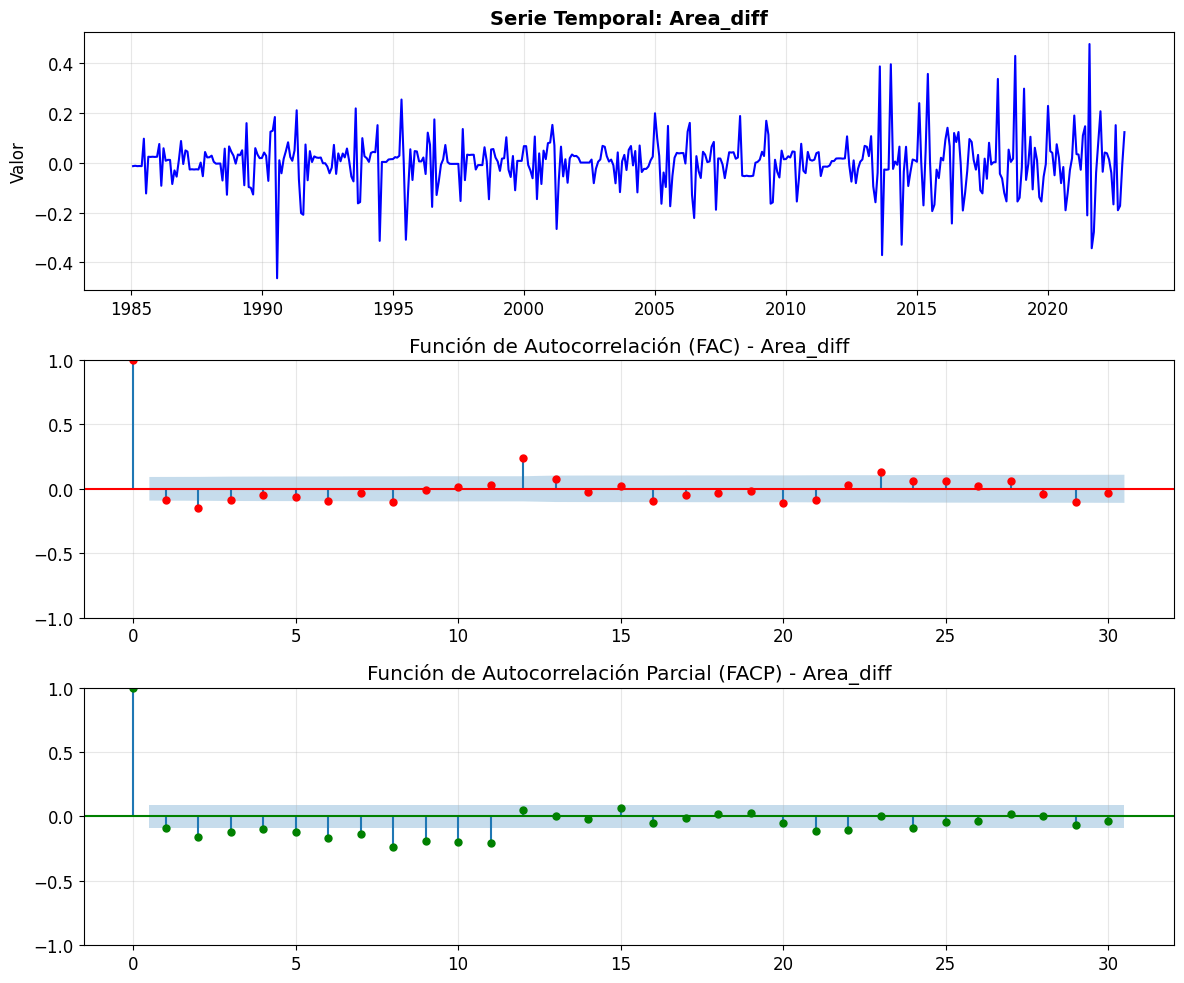
\includegraphics[scale=.42]{Figures/facp_Area_dif.png}
    \caption{Funciones ACF y PACF de la serie Área (superficie de agua).}
    \label{fig:facp_area_dif}
\end{figure}

\begin{table}[H]
    \centering
    \caption{Resultados de pruebas de estacionariedad aplicadas a Área\_diff}
    \label{tab:ru_area_diff}
    \begin{tabular}{lccc}
        \toprule
        \textbf{Prueba} & \textbf{Estadístico} & \textbf{p-valor} & \textbf{Conclusión} \\
        \midrule
        Dickey-Fuller Aumentada (ADF) & -14.8466 & 0.0000 & Estacionaria \\
        KPSS & 0.0239 & 0.1000 & Estacionaria \\
        Phillips-Perron (PP) & -33.5219 & 0.0000 & Estacionaria \\
        \bottomrule
    \end{tabular}
\end{table}

Las tres pruebas (ADF, KPSS y PP) coinciden en rechazar la hipótesis de no estacionariedad, 
confirmando que la serie diferenciada es estacionaria. Este resultado valida la 
necesidad del preprocesamiento y garantiza que la serie Área\_diff puede ser utilizada en 
modelos ARIMA o SARIMA con mayor robustez. 


\section{Modelado con SARIMA}

El modelo SARIMA (\textit{Seasonal ARIMA}) fue optimizado para cada una de las series de interés (ONI, SOI, MEI y Área), evaluando diferentes combinaciones de parámetros $(p,d,q)\times(P,D,Q,s)$ y seleccionando los mejores ajustes según el criterio de información de Akaike (AIC). 

\subsection{ONI}
El mejor modelo seleccionado para ONI fue SARIMA$(2,0,1)\times(1,1,2)_{12}$, con un AIC de $-410.64$. Este modelo supera en desempeño a alternativas cercanas como SARIMA$(2,0,2)\times(1,1,2)_{12}$ y SARIMA$(2,0,0)\times(1,1,2)_{12}$, confirmando que la estructura óptima incluye un componente autorregresivo de orden 2 y un componente de media móvil de orden 1.

\subsection{SOI}
En el caso de SOI, el mejor modelo corresponde a SARIMA$(1,0,2)\times(2,1,2)_{12}$, con un AIC de $2842.34$. Aunque este valor absoluto es elevado (debido a la alta varianza intrínseca de la serie), la comparación relativa muestra que es la configuración más adecuada frente a otras alternativas con órdenes similares.

\subsection{MEI}
La serie MEI fue mejor explicada por SARIMA$(2,0,2)\times(1,1,2)_{12}$, alcanzando un AIC de $126.37$. Este modelo captura tanto la persistencia como los patrones estacionales de la serie, y presenta una ventaja clara frente a otros candidatos como SARIMA$(1,0,1)\times(1,1,2)_{12}$ y SARIMA$(2,0,1)\times(1,1,2)_{12}$.

\subsection{Área y Área\_diff}
Para la serie Área sin diferenciar, el mejor modelo fue SARIMA$(1,0,0)\times(1,0,1)_{12}$ con un AIC de $-902.08$. Sin embargo, al diferenciar la serie (Área\_diff), se obtuvo como mejor ajuste el modelo SARIMA$(2,0,1)\times(1,0,1)_{12}$ con un AIC de $-888.19$. Aunque el AIC es ligeramente menos favorable tras la diferenciación, los análisis de raíces unitarias y métricas de predicción (ver subsección anterior) mostraron que el modelo diferenciado ofrece mayor robustez y estacionariedad.

\begin{table}[H]
    \centering
    \caption{Resumen de los mejores modelos SARIMA seleccionados por serie}
    \begin{tabular}{lccc}
        \toprule
        \textbf{Serie} & \textbf{Mejor modelo SARIMA} & \textbf{AIC} & \textbf{Notas} \\
        \midrule
        ONI   & $(2,0,1)\times(1,1,2)_{12}$ & $-410.64$ & Estacionalidad marcada \\
        SOI   & $(1,0,2)\times(2,1,2)_{12}$ & $2842.34$ & Alta varianza residual \\
        MEI   & $(2,0,2)\times(1,1,2)_{12}$ & $126.37$  & Buen equilibrio AR y MA \\
        Área  & $(1,0,0)\times(1,0,1)_{12}$ & $-902.08$ & No diferenciada \\
        Área\_diff & $(2,0,1)\times(1,0,1)_{12}$ & $-888.19$ & Estacionaria, mayor robustez \\
        \bottomrule
    \end{tabular}
    \label{tab:sarima_modelos}
\end{table}

En síntesis, el procedimiento de optimización permitió identificar configuraciones distintas para cada serie, adaptadas a sus características temporales. En los siguientes apartados se evaluará la performance predictiva de estos modelos sobre los conjuntos de test.

\section{Evaluación de los modelos SARIMA}

Se evaluó el desempeño predictivo de los modelos SARIMA seleccionados para las series
ONI, SOI, MEI, \emph{Área} y \emph{Área\_diff}, considerando: (i) métricas de error en el
conjunto de test (MSE, MAE, RMSE y MAPE cuando aplica), (ii) diagnóstico de residuos
(residuos en el tiempo, ACF/PACF de residuos, normalidad aproximada y test de Ljung--Box),
y (iii) parsimonia y significancia de coeficientes (AIC/BIC, $p$--valores).

\subsection{Criterios de diagnóstico}
Se consideró que un modelo es adecuado cuando (a) los residuos no presentan
autocorrelación remanente (ACF/PACF dentro de bandas y Ljung--Box con $p>0.05$), (b) no hay
patrones sistemáticos en los residuos, (c) las métricas de error son coherentes con la
escala de la serie, y (d) la parametrización es parsimoniosa (sin términos
innecesarios o no significativos).

\subsection{Resultados por serie y diagnóstico}
Para cada serie se incluyen: (i) residuos en el tiempo, (ii) ACF y PACF de residuos,
(iii) histograma, densidad y Q–Q plot, (iv) gráfico de p--valores de Ljung--Box por lag,
y (v) observados (train+test) vs. predicciones con IC 95\%. Todos estos gráficos pueden verse en el Apéndice de figuras. 

\subsubsection{ONI} 
Modelo SARIMA$(2,0,1)\times(1,1,2)_{12}$ (AIC $\approx -410.6$). 
Los coeficientes no estacionales AR(2) y MA(1) son altamente significativos y capturan la
dinámica de corto plazo; sin embargo, los \emph{términos estacionales} no resultan
significativos. El test Jarque--Bera rechaza normalidad y se observa heterocedasticidad,
pero los residuos no presentan autocorrelación relevante. En test: 
MSE $=0.683$, MAE $=0.631$, RMSE $=0.826$ (MAPE no informativo por valores próximos a cero).
\emph{Conclusión:} buen ajuste de la dinámica no estacional; recomendable
simplificar la parte estacional (evaluar ARIMA$(2,0,1)$ sin estacionalidad) y re‐chequear
residuos.
\vspace{0.3em}

\begin{figure}[H]\centering
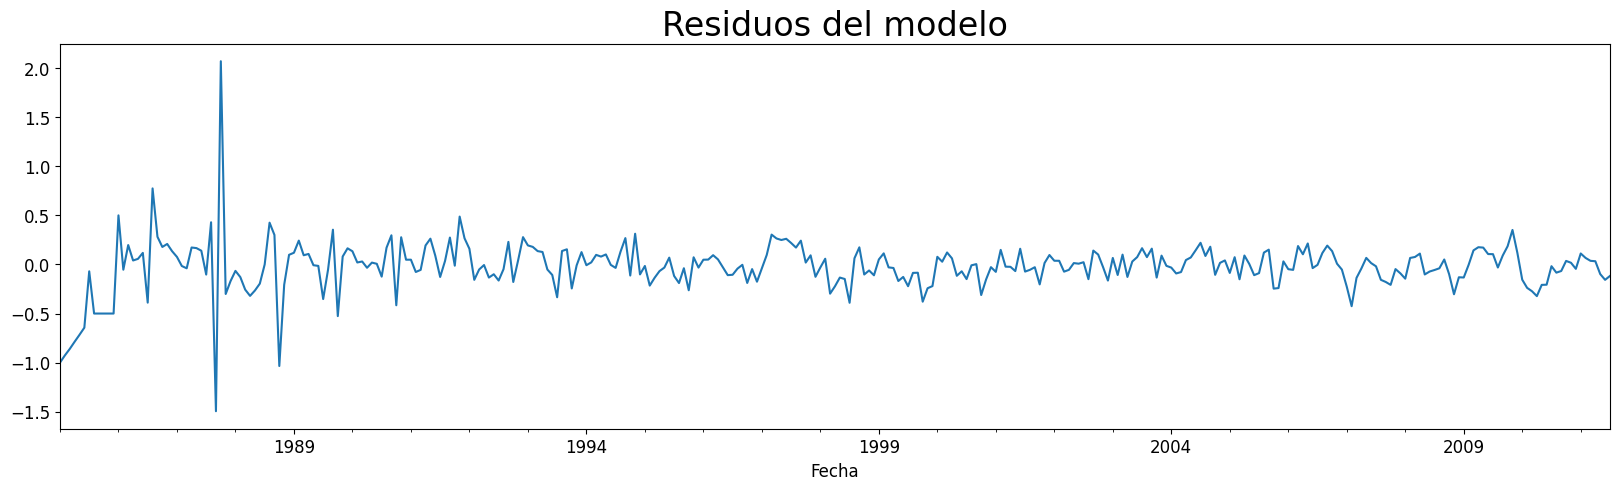
\includegraphics[scale=.30]{Figures/res_sarima_oni.png}
\caption{ONI: residuos del modelo SARIMA.}
\label{fig:res_oni}
\end{figure}

\begin{figure}[H]\centering
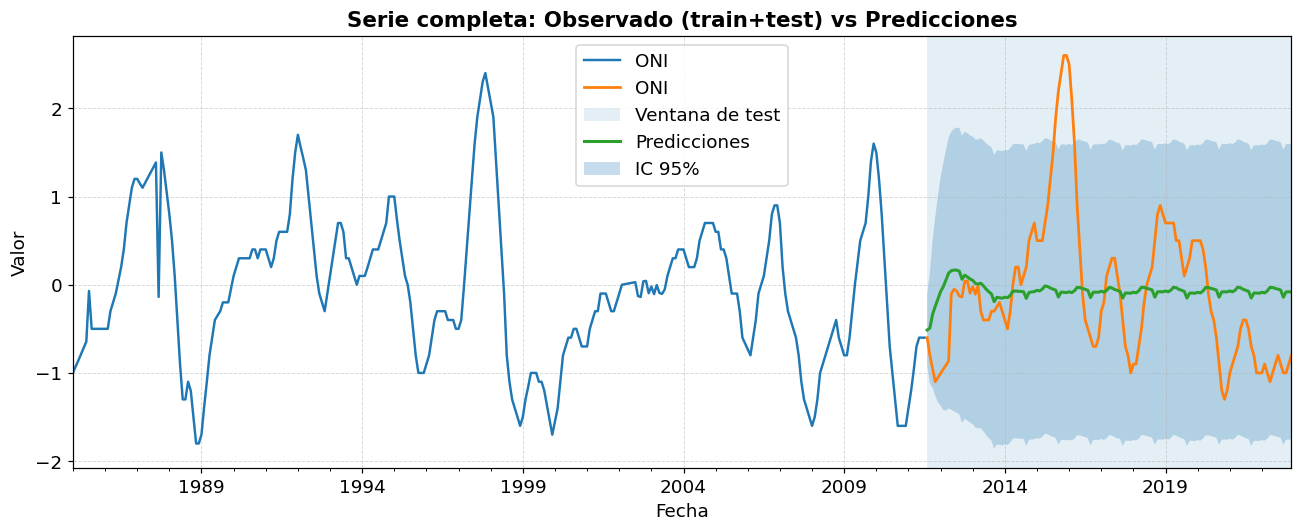
\includegraphics[scale=.42]{Figures/pred_oni.png}
\caption{ONI: observado (train+test) vs. predicciones con IC 95\%.}
\label{fig:pred_oni}
\end{figure}


\subsubsection{SOI}
Modelo SARIMA$(1,0,2)\times(2,1,2)_{12}$ (AIC $\approx 2116$).
AR(1), MA(1) y varios términos estacionales son significativos; MA(2) y AR estacional en
$24$ meses no lo son. Residuos sin autocorrelación (Ljung--Box con $p>0.05$) y con leve
no normalidad. En test: MSE $=88.00$, MAE $=7.64$, RMSE $=9.38$ (MAPE no informativo).
\emph{Conclusión:} desempeño predictivo \textbf{insuficiente} para la escala del SOI; conviene
\emph{simplificar} (eliminar términos no significativos), explorar \emph{transformaciones
robustas} (p.\,ej., winsorización) y/o considerar modelos alternativos (ARIMA con
diferenciación adicional, modelos con heterocedasticidad, o enfoques no lineales).
\vspace{0.3em}

\begin{figure}[H]\centering
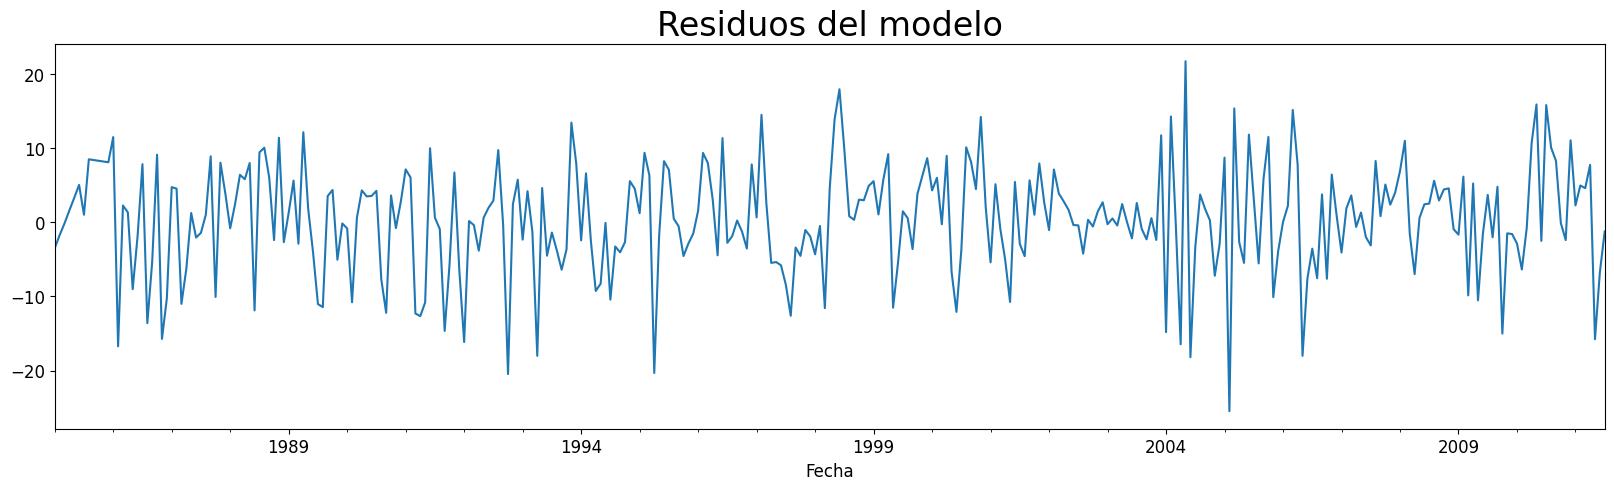
\includegraphics[scale=.30]{Figures/res_sarima_soi.png}
\caption{SOI: residuos del modelo SARIMA.}
\label{fig:res_soi}
\end{figure}


\begin{figure}[H]\centering
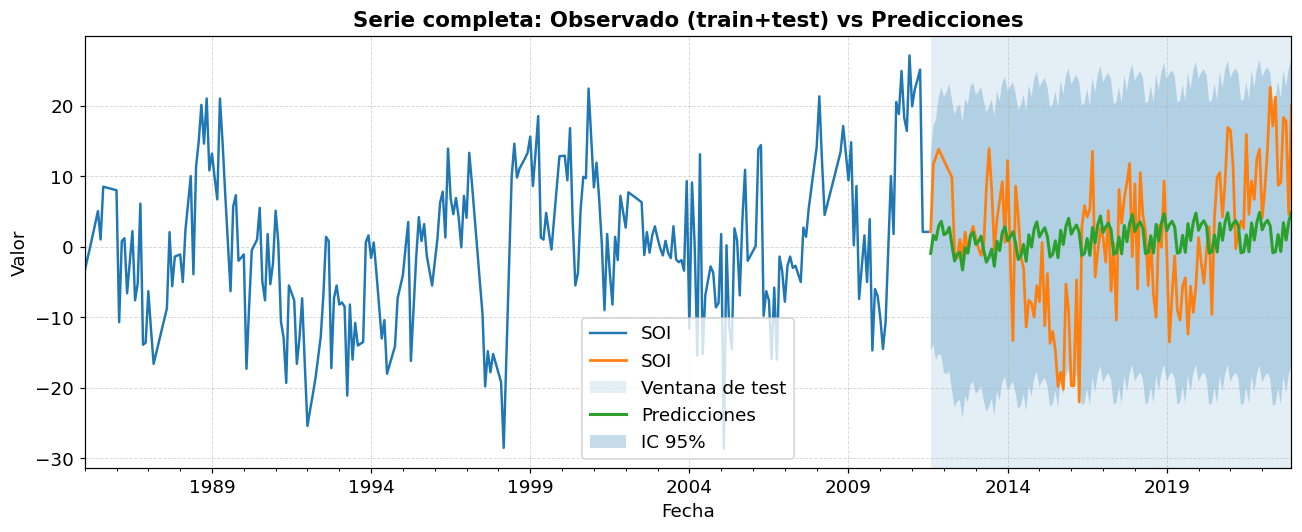
\includegraphics[scale=.42]{Figures/pred_soi.png}
\caption{SOI: observado (train+test) vs. predicciones con IC 95\%.}
\label{fig:pred_soi}
\end{figure}


\subsubsection{MEI}
Modelo SARIMA$(2,0,2)\times(1,1,2)_{12}$ (AIC $\approx 126.4$).
AR(1), AR(2) y MA(1) no estacionales son muy significativos; el MA(2) es marginal. 
En la parte estacional sólo AR a 12 meses es relevante; los términos MA estacionales no lo son.
Residuos sin autocorrelación (Ljung--Box con $p\approx 0.84$), con colas algo pesadas.
En test: MSE $=0.821$, MAE $=0.725$, RMSE $=0.906$ (MAPE no informativo).
\emph{Conclusión:} \textbf{buen comportamiento predictivo}; se sugiere \emph{simplificar}
la estacionalidad (p.\,ej., SARIMA$(2,0,1)\times(1,1,0)_{12}$) y verificar residuos.
\vspace{0.3em}

\begin{figure}[H]\centering
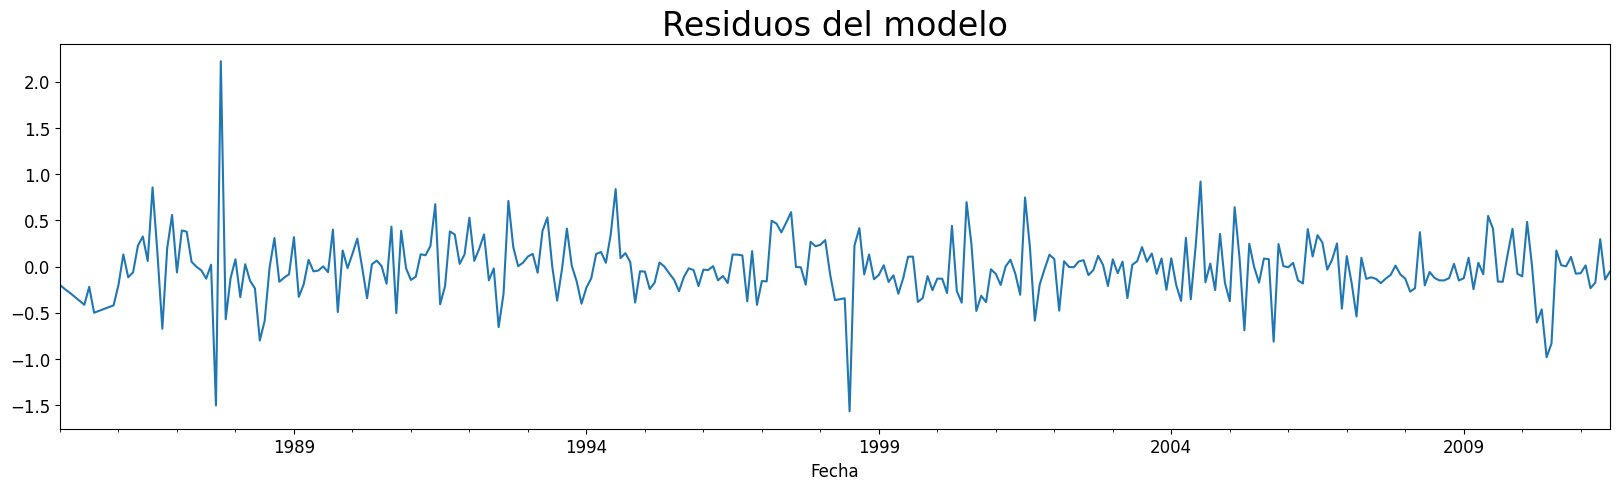
\includegraphics[scale=.30]{Figures/res_sarima_mei.png}
\caption{MEI: residuos del modelo SARIMA.}
\label{fig:res_mei}
\end{figure}


\begin{figure}[H]\centering
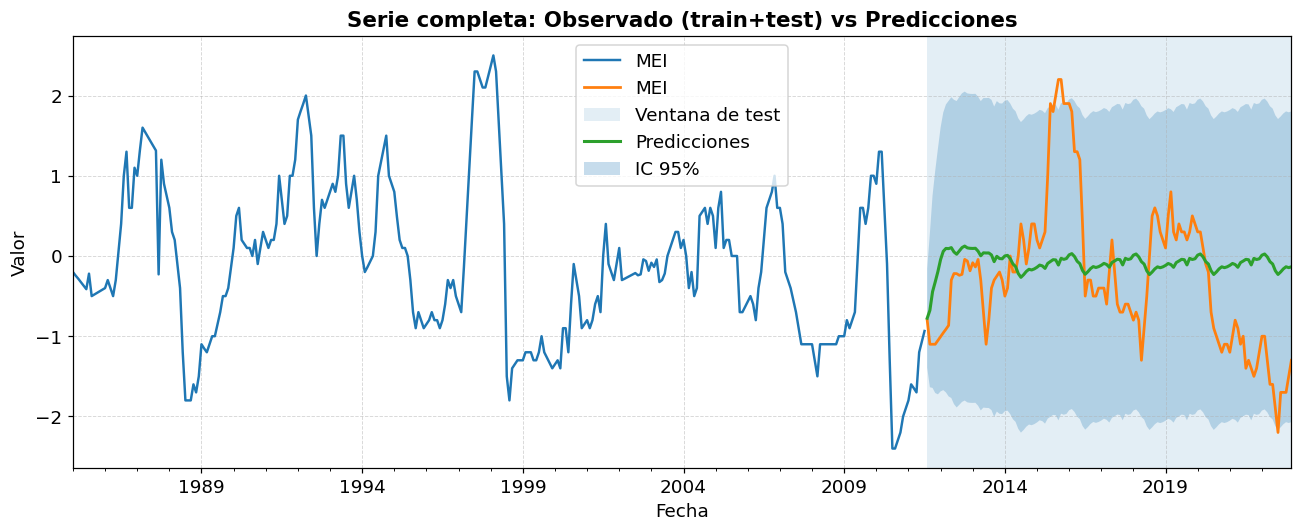
\includegraphics[scale=.42]{Figures/pred_mei.png}
\caption{MEI: observado (train+test) vs. predicciones con IC 95\%.}
\label{fig:pred_mei}
\end{figure}


\subsubsection{Área (sin diferenciar)}
Modelo SARIMA$(1,0,0)\times(1,0,1)_{12}$ 
(AIC $\approx -902.1$). Todos los coeficientes son significativos; el término AR estacional
es muy alto ($\approx 0.996$), lo que sugiere posible necesidad de diferenciación
estacional. Residuos sin autocorrelación, aunque con no normalidad (colas pesadas).
En test: MSE $=0.02499$, MAE $=0.119$, RMSE $=0.158$ (MAPE no informativo).
\emph{Conclusión:} ajuste \textbf{excelente} en escala de la serie; aun así, la magnitud de
AR estacional invita a evaluar un $D=1$ si se buscara mayor estabilidad.
\vspace{0.3em}

\begin{figure}[H]\centering
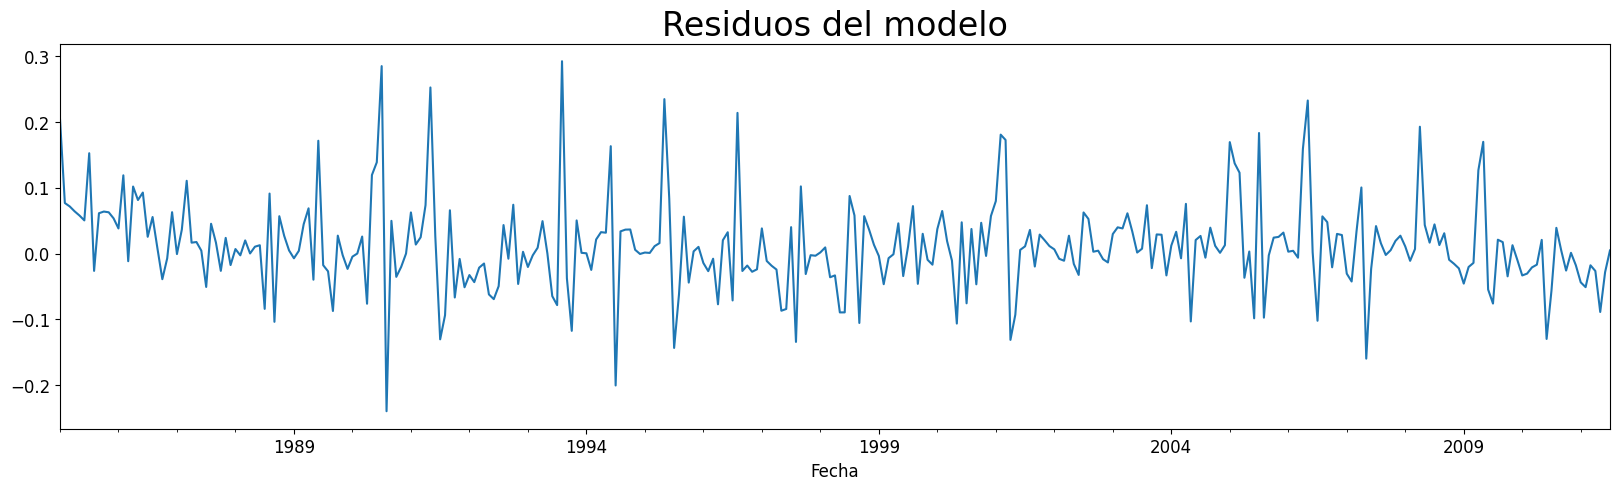
\includegraphics[scale=.30]{Figures/res_sarima_area.png}
\caption{Área: residuos del modelo SARIMA.}
\label{fig:res_area}
\end{figure}



\begin{figure}[H]\centering
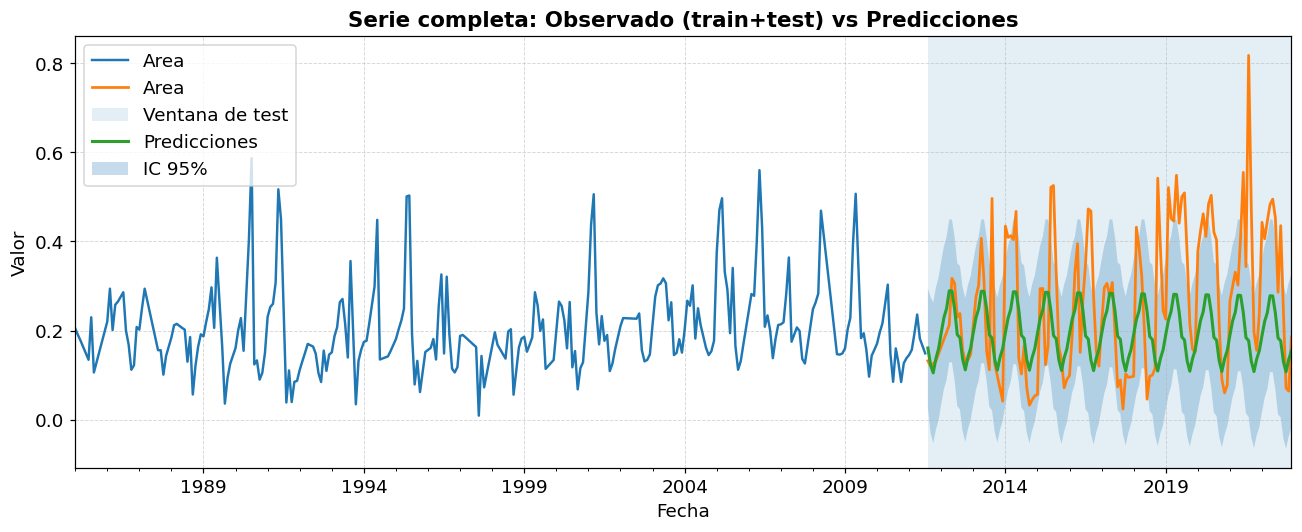
\includegraphics[scale=.42]{Figures/pred_area.png}
\caption{Área: observado (train+test) vs. predicciones con IC 95\%.}
\label{fig:pred_area}
\end{figure}


\subsubsection{Área\_diff (diferenciada)}
Modelo SARIMA$(2,0,1)\times(1,0,1)_{12}$
(AIC $\approx -888.2$). Residuos con comportamiento de ruido blanco (ACF/PACF dentro
de bandas, Ljung--Box con $p>0.05$), normalidad aproximada y métricas de error muy bajas:
MSE $=0.01782$, MAE $=0.0910$, RMSE $=0.1335$, MAPE $=1.70\%$. 
\emph{Conclusión:} \textbf{desempeño sobresaliente} y mayor robustez estadística tras la
diferenciación; valida el preprocesamiento efectuado (ver sección de raíces unitarias).

\begin{figure}[H]\centering
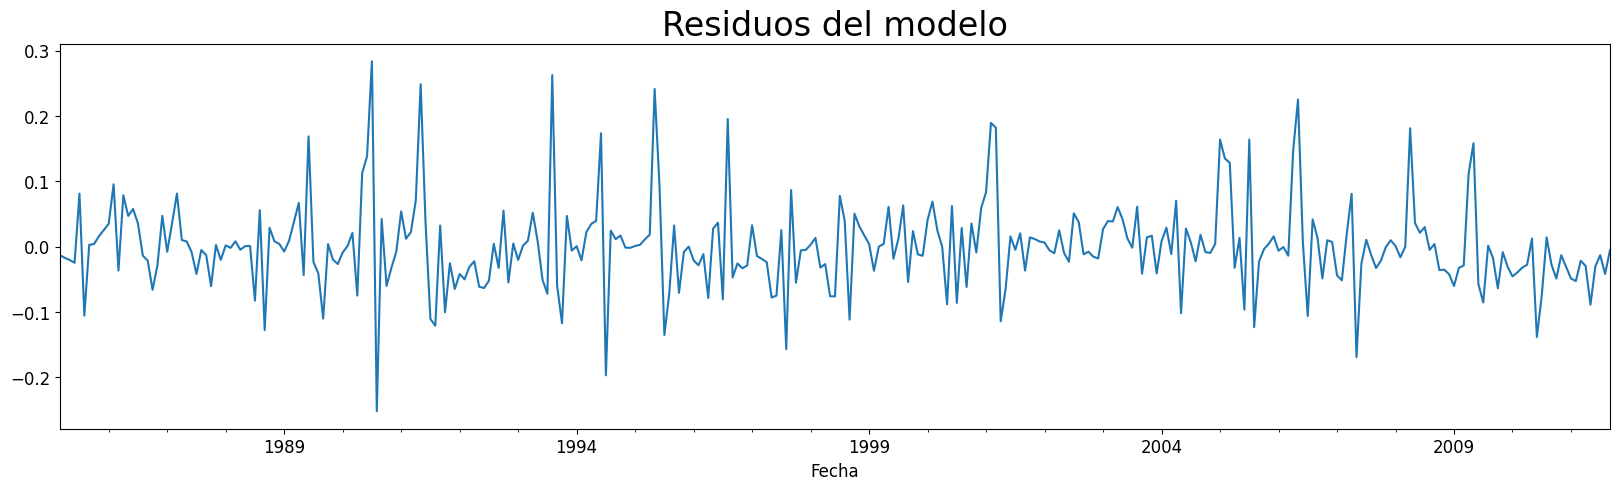
\includegraphics[scale=.30]{Figures/res_sarima_area_d.png}
\caption{Área (diferenciada): residuos del modelo SARIMA.}
\label{fig:res_area_d}
\end{figure}


\begin{figure}[H]\centering
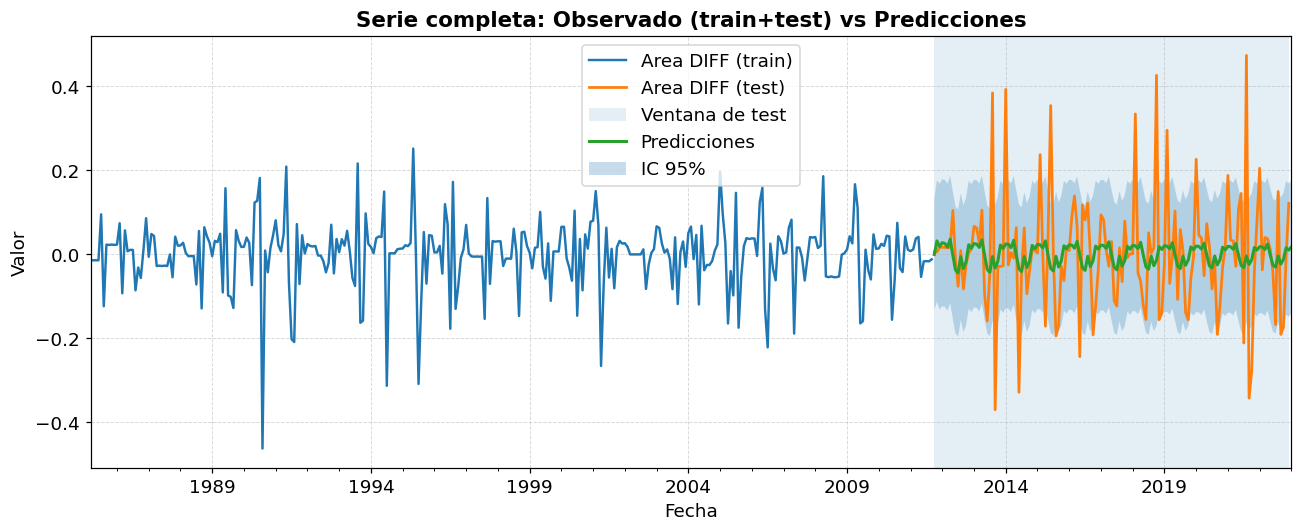
\includegraphics[scale=.42]{Figures/pred_area_d.png}
\caption{Área (diferenciada): observado (train+test) vs. predicciones con IC 95\%.}
\label{fig:pred_area_d}
\end{figure}





\subsection{Métricas comparativas (conjunto de test)}
\begin{table}[H]
\centering
\caption{Resumen de métricas de desempeño en test para modelos SARIMA}
\label{tab:metricas_sarima}
\begin{tabular}{lcccc}
\toprule
\textbf{Serie} & \textbf{MSE} & \textbf{MAE} & \textbf{RMSE} & \textbf{MAPE} \\
\midrule
ONI  & 0.683  & 0.631  & 0.826  & n/a \\
SOI  & 88.003 & 7.639  & 9.381  & n/a \\
MEI  & 0.821  & 0.725  & 0.906  & n/a \\
Área (sin diff) & 0.02499 & 0.1190 & 0.1581 & n/a \\
Área\_diff      & \textbf{0.01782} & \textbf{0.0910} & \textbf{0.1335} & \textbf{1.70\%} \\
\bottomrule
\end{tabular}
\end{table}

\paragraph{Síntesis y recomendaciones}
\begin{itemize}
    \item Series ENSO (ONI, MEI): los componentes AR(2) y MA(1) no estacionales
    capturan bien la memoria de corto plazo; varios términos MA estacionales no son
    significativos. \emph{Recomendación:} simplificar la parte estacional y revalidar
    residuos (p.\,ej., ONI $\to$ ARIMA$(2,0,1)$; MEI $\to$ SARIMA$(2,0,1)\times(1,1,0)_{12}$).
    \item SOI: las métricas son altas; aunque los residuos no muestran
    autocorrelación, la precisión predictiva es pobre. \emph{Recomendación:} simplificar
    (remover términos no significativos), explorar transformaciones robustas y/o modelos
    alternativos (p.\,ej., errores heterocedásticos o modelos no lineales).
    \item Área vs. Área\_diff: ambos modelos presentan muy buen desempeño en test,
    destacándose \emph{Área\_diff} con los errores más bajos y residuos más
    estables. \emph{Recomendación:} usar \emph{Área\_diff} para pronóstico operativo; 
    documentar que el nivel se obtiene por acumulación inversa si se requiere volver a
    escala original.
\end{itemize}


En conjunto, la evidencia empírica muestra que la diferenciación de la serie \emph{Área}
mejora la robustez y precisión del modelo, mientras que en las series ENSO una
parametrización más parsimoniosa tiende a ser suficiente. El caso SOI requiere trabajo
adicional para alcanzar niveles de error aceptables.

\section{Modelado VAR (Vectores Autorregresivos)}

El modelo VAR (\textit{Vector AutoRegressive}) es una técnica de series temporales multivariadas que permite capturar las interdependencias entre varias variables a lo largo del tiempo. A diferencia de los modelos univariados como ARIMA o SARIMA, el VAR considera que cada variable del sistema depende no solo de sus propios valores pasados, sino también de los valores pasados de las demás variables incluidas en el modelo \parencite{lutkepohl2005new}.

En este estudio se incluyeron cuatro series temporales: los índices climáticos ONI, SOI y MEI, y la superficie de agua (Área). Todas las series fueron previamente transformadas para garantizar estacionariedad mediante diferenciación y pruebas de raíz unitaria (ADF, KPSS y PP). Posteriormente, se seleccionó el número óptimo de rezagos considerando los criterios de información (AIC, BIC y HQIC), con un máximo de 24 meses de retraso para capturar los efectos interanuales asociados a la variabilidad ENSO.

El análisis VAR constituye la base para explorar relaciones causales entre las variables y evaluar la capacidad predictiva conjunta del sistema.

\subsection{Prueba de Causalidad de Granger}

La prueba de causalidad de Granger evalúa si los valores pasados de una serie temporal contienen información útil para predecir otra serie, bajo el supuesto de relaciones lineales dentro de un modelo VAR \parencite{granger1969investigating}.
La hipótesis nula (\(H_0\)) establece que “la serie X no causa Granger a la serie Y”. Un p-valor inferior a 0.05 permite rechazar la hipótesis nula, concluyendo que existe causalidad grangeriana.

En este estudio, se aplicó la prueba con un máximo de 24 rezagos mensuales, obteniéndose la matriz de resultados presentada en la Tabla~\ref{tab:granger_matrix}.

\begin{table}[H]
    \centering
    \caption{Matriz de p-valores de la prueba de causalidad de Granger (máx. 24 rezagos).}
    \label{tab:granger_matrix}
    \begin{tabular}{lcccc}
        \toprule
        & ONI\_x & SOI\_x & MEI\_x & Área\_x \\
        \midrule
        ONI\_y  & 0.9999   & 0.1189   & 0.0142$^{*}$ & 0.1057   \\
        SOI\_y  & 0.0000$^{*}$ & 1.0000   & 0.0000$^{*}$ & 0.0410$^{*}$ \\
        MEI\_y  & 0.0000$^{*}$ & 0.0000$^{*}$ & 1.0000   & 0.3261   \\
        Área\_y & 0.5889   & 0.0456$^{*}$ & 0.4557   & 1.0000   \\
        \bottomrule
    \end{tabular}
    
    \begin{flushleft}
    {\footnotesize Nota: $^{*}$ indica significancia estadística al 5\%.}
    \end{flushleft}
\end{table}

\subsubsection{Interpretación de resultados:}

\begin{itemize}
    \item ONI\_y: sólo es causado por el MEI (p=0.014), lo que indica que la información del índice multivariado MEI contribuye a predecir al ONI.
    \item SOI\_y: recibe causalidad de ONI, MEI y el Área, reflejando su carácter central como índice atmosférico.
    \item MEI\_y: es causado por ONI y SOI, lo que confirma la fuerte interdependencia entre los índices climáticos de ENSO.
    \item Área\_y: solo es causada por el SOI (p=0.046), lo que evidencia que la variabilidad atmosférica influye directamente en la superficie de agua del salar.
\end{itemize}



\subsubsection{Conclusiones}  
El análisis de causalidad de Granger confirma la interdependencia entre los tres índices climáticos (ONI, SOI, MEI), coherente con la naturaleza multivariada del ENSO. Entre ellos, el \textbf{SOI emerge como el índice más influyente}, pues no solo se ve afectado por ONI y MEI, sino que además es el único que causa variaciones significativas en el área de agua superficial. Este hallazgo refuerza la hipótesis de que la dinámica atmosférica vinculada al SOI constituye un modulador clave de la hidrología altoandina.

\subsection{Modelo VAR: Selección del orden y resultados}

Para modelar la dinámica conjunta entre los índices ENSO (ONI, SOI, MEI) y la superficie de agua (\textit{Área}), se ajustó un modelo VAR (Vector Autorregresivo). A diferencia de los modelos univariados como ARIMA o SARIMA, el VAR permite capturar relaciones dinámicas multivariadas, considerando que cada variable depende tanto de sus propios rezagos como de los rezagos de las demás variables del sistema \cite{lutkepohl2005new}.

\subsubsection{Selección del orden de rezagos}
Se evaluaron los criterios de información AIC, BIC, HQIC y FPE para determinar el número óptimo de rezagos (Tabla~\ref{tab:var_lags}). Los resultados muestran que el rezago $p=3$ minimiza la mayoría de los criterios (AIC, HQIC y FPE), por lo que se seleccionó un modelo VAR(3).

\begin{table}[H]
    \centering
    \caption{Selección del orden de rezagos para el modelo VAR.}
    \label{tab:var_lags}
    \begin{tabular}{lcccc}
        \toprule
        \textbf{Rezago} & \textbf{AIC} & \textbf{BIC} & \textbf{HQIC} & \textbf{FPE} \\
        \midrule
        2 & -7.485 & -7.130$^\ast$ & -7.345 & 0.0005612 \\
        3 & -7.617$^\ast$ & -7.104 & -7.414$^\ast$ & 0.0004921$^\ast$ \\
        \bottomrule
    \end{tabular}
\end{table}

\subsubsection{Resultados del VAR(3)}
El ajuste del modelo mostró que:

\begin{itemize}
    \item ONI presenta un fuerte componente autoregresivo, con significancia en los rezagos 1 y 3, lo que confirma su persistencia temporal.
    \item SOI depende de sus propios rezagos, pero también recibe influencia significativa del ONI, reforzando los vínculos entre estos índices ENSO.
    \item MEI es explicado principalmente por sus propios rezagos, aunque también recibe influencia de ONI y SOI.
    \item El Área muestra alta dependencia de su propio rezago inmediato (L1.Area $\approx 0.67$), lo que indica fuerte persistencia temporal. Además, se observa una influencia marginal de SOI (p≈0.05), consistente con la prueba de causalidad de Granger.
\end{itemize}

\subsubsection{Matriz de correlación de residuos}
La matriz de correlación entre los residuos (Tabla~\ref{tab:var_corr_resid}) muestra que:

\begin{itemize}
    \item ONI y MEI presentan una correlación positiva alta (0.59), consistente con la interdependencia observada en los coeficientes.
    \item SOI mantiene correlaciones negativas con ONI (-0.23) y MEI (-0.45), reforzando su rol como índice atmosférico diferenciado.
    \item El Área muestra correlaciones débiles con el resto de variables, lo que indica que sus residuos son relativamente independientes.
\end{itemize}


\begin{table}[H]
    \centering
    \caption{Matriz de correlación de los residuos del modelo VAR(3).}
    \label{tab:var_corr_resid}
    \begin{tabular}{lcccc}
        \toprule
               & ONI & SOI & MEI & Área \\
        \midrule
        ONI     & 1.000 & -0.232 &  0.590 &  0.068 \\
        SOI     & -0.232 & 1.000 & -0.454 & -0.094 \\
        MEI     & 0.590 & -0.454 &  1.000 &  0.066 \\
        Área    & 0.068 & -0.094 &  0.066 &  1.000 \\
        \bottomrule
    \end{tabular}
\end{table}

\subsubsection{Normalidad de los residuos}
Se aplicó el test de normalidad basado en asimetría y curtosis. La hipótesis nula (H$_0$: residuos con distribución normal) fue rechazada al 5\% de significancia (p-valor=0.000). Esto indica que los residuos no son normales, presentando colas pesadas y asimetrías, una situación común en series climáticas y ambientales. Aunque no compromete la validez del VAR, sí implica que los intervalos de confianza deben interpretarse con cautela.

\subsubsection{Predicciones}
En la Figura~\ref{fig:var_pred} se presentan las predicciones del modelo VAR comparadas con los valores observados. Se observa que el modelo logra capturar adecuadamente la evolución de ONI y MEI, mientras que en SOI las oscilaciones extremas resultan más difíciles de reproducir. En el caso del Área, las predicciones se mantienen dentro de un rango consistente, aunque con menor variabilidad que la observada.

\begin{figure}[H]
    \centering
    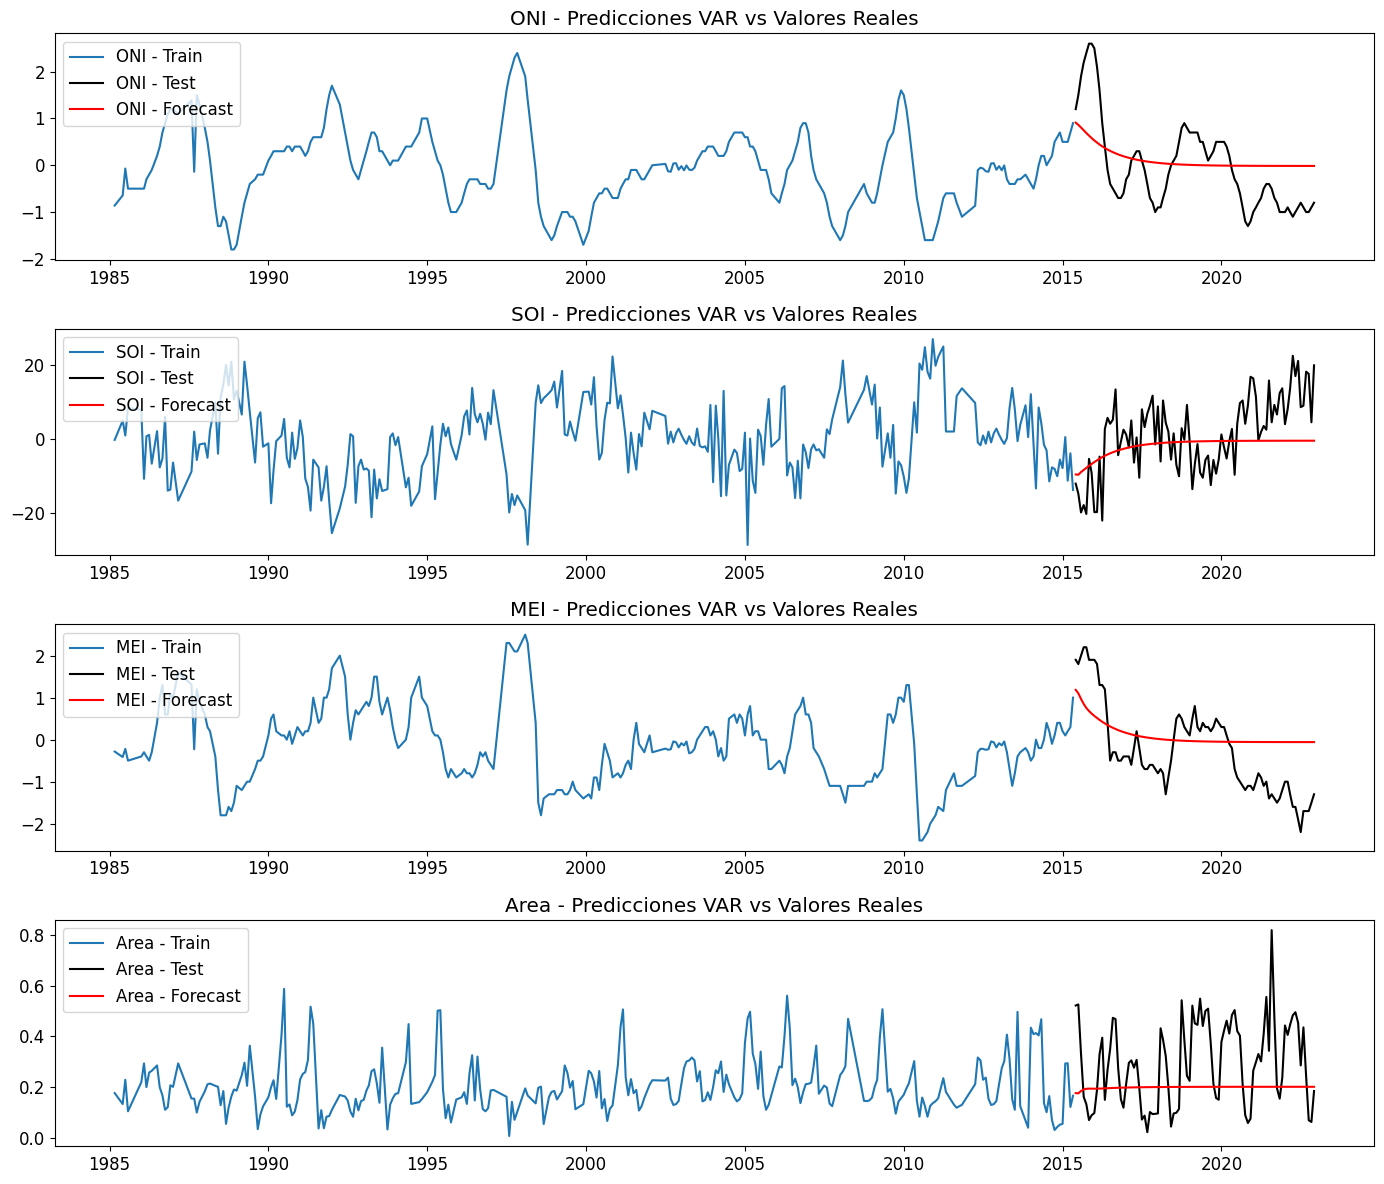
\includegraphics[scale=0.45]{Figures/var_pred.png}
    \caption{Predicciones del modelo VAR(3) frente a los valores reales de ONI, SOI, MEI y Área.}
    \label{fig:var_pred}
\end{figure}

\subsubsection{Respuestas al impulso}
Las funciones de respuesta al impulso (IRF) permiten evaluar cómo un shock en una variable afecta a las demás dentro del sistema (Figura~\ref{fig:var_irf}). Los resultados indican que:

\begin{itemize}
    \item Un shock positivo en ONI genera efectos persistentes en sí mismo y también incrementa los valores de MEI.
    \item Un shock en SOI produce impactos negativos significativos sobre ONI y MEI, además de afectar el Área en los primeros periodos.
    \item El Área responde principalmente a perturbaciones de SOI, lo que refuerza su rol como variable climática clave que influye en la superficie de agua.
\end{itemize}


\begin{figure}[H]
    \centering
    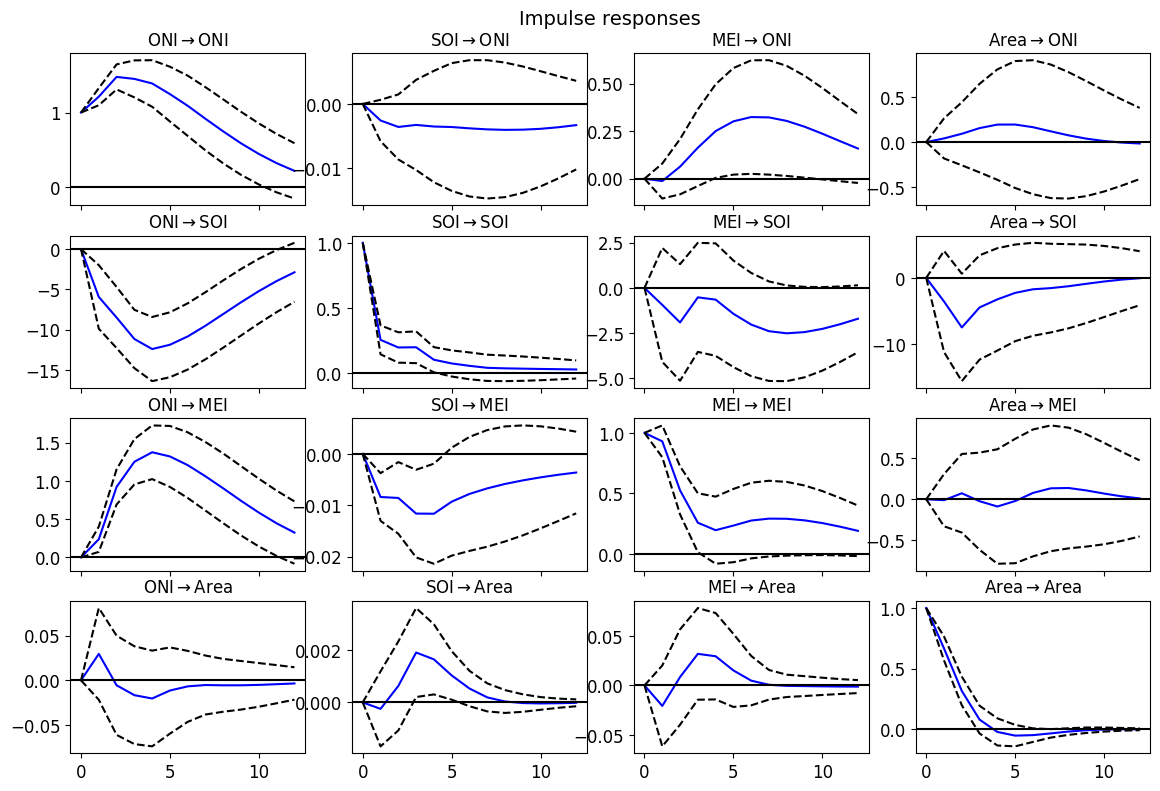
\includegraphics[scale=0.45]{Figures/var_ir.png}
    \caption{Funciones de respuesta al impulso (IRF) para el modelo VAR(3).}
    \label{fig:var_irf}
\end{figure}

\subsubsection{Conclusión parcial}
El modelo VAR(3) confirma la fuerte interrelación entre los índices ENSO (ONI, SOI, MEI) y muestra que la superficie de agua está particularmente influenciada por el SOI. Este resultado es consistente con la prueba de causalidad de Granger y con la lógica climática subyacente: la variabilidad atmosférica medida por el SOI tiene un efecto directo en la dinámica hidrológica del sistema estudiado. No obstante, la no normalidad de los residuos sugiere que futuros trabajos deberían considerar modelos más robustos (ej. VAR-GARCH o VAR con errores no gaussianos).


